\chapter{Case Studies in English Diachrony}\label{ch:diachron}
\section{Introduction}
This chapter studies the claims presented in the previous three chapters with two case studies in the development of recipient ditransitive syntax in the history of English. As discussed in the introduction, quantitative (and especially) diachronic studies can provide a useful independent verification of analyses developed on the basis of acceptability judgements. Crucially, data from systematic patterns in language production can provide independent verification of theories developed primarily from language comprehension (i.e., acceptability judgements).

Theoretical linguistics has a problem (common to the social sciences) of finding empirical validations for theoretical claims. Building on the work starting during the cognitive revolution in the 50s and 60s, the goal of generative linguistics has been to study the linguistic competence of speakers, which consists of the language specific information that is needed to use a language natively \citep{Chomsky.1981,Chomsky.1986}. As will be shown below (in particular when looking at passivisation), this linguistic competence can be separated into grammatical and non-grammatical competences. This distinction between grammatical and non-grammatical competences depends on a specific notion of grammar.

A grammar can be thought of as a list of the possible sound--meaning pairs in a language. Since at least \cite{Chomsky.1957}, it has been recognised that this list is infinitely long for any natural language (because of the recursive nature of natural language). The generative grammar program has endeavoured to describe a set of finite rules which are capable of generating the correct sound--meaning pairs. Often, an even simpler goal is attempted, namely to separate strings (chunks of sound) into two sets: (a) the strings that have at least one meaning associated with them (grammatical strings) and (b) the strings that have no meaning associated with them (ungrammatical strings). Note that these meanings do not need to plausibly arise in actual discourse; all that is necessary for a string to be grammatical is that it have \textbf{some} meaning associated with it.\footnote{The classic example from Chomsky's work is ``Colourless green ideas sleep furiously'', which certainly has no real world referent, but is grammatical and has a meaning associated with it (simply a nonsensical meaning). Given that contradictions are stateable in natural languages, whatever our definition of meaning is for grammaticality, it must be able to include nonsensical meanings. That these meanings are truth conditionally equivalent, but yet are felt to be distinct for speakers (e.g., ``Both A and not A'' and ``X equals 1 and not 1'' are both contradictions, but have different meanings), suggests that natural language meaning is fundamentally intensional rather than extensional.}

Given the rampant ambiguity in natural language, the grammar of natural languages often associates multiple strings with the same meaning (and multiple meanings with the same string). Since the purpose of the grammar is to simply list whether a string is associated with an utterance, it cannot help a speaker decide which string to use in production from among the set of strings compatible with the meaning they are trying to express. This problem of knowing which of the options produced by the grammar to use in any particular circumstance is an equally important part of any native speakers linguistic competence. These choices are often impacted by language specific implementations of general social or psychological factors (see \cite{Bresnan.2007,Bresnan.2010,Zeevat.2014} and \cite{Tamminga.2016} for a discussion of these issues and their relationship to the grammar). These choices can be formalised as representing probability distributions over the forms provided for by the grammar.

Given that such probability distributions need to exist (in order for speakers to use language), it is worthwhile to discuss what properties they might have. These choices often depend on specific properties of the strings in questions (e.g., on the prosodic heaviness of certain arguments for determining the likelihood of Heavy NP shift). Therefore, the same logic that motivated adopting generative approaches to grammar (i.e., the impossibility of simply listing the grammatical/ungrammatical pairings) applies here. It would be impossible to simply memorise the relevant probability distributions, since they apply (and are affected by properties of) an infinite number of strings. Thus, a generative mechanism for producing probability distributions for any given set of grammatical alternatives is necessary.

Unfortunately, it has been known since the beginning of the generative grammar enterprise that there is no direct evidence of linguistic competence (see \cite{Schutze.1996} for a discussion of early claims about this issue), which is typical of knowledge and psychological constructs. Instead, it has been necessary to deduce the nature of the linguistic knowledge by studying its effects on language performance (see \citealt{Stroud.2012,Phillips.2013, Phillips.2013b, Phillips.2013c} for an arguments that acceptability judgements are fundamentally performative).

One of the most prominent types of linguistic performance to be used in theoretical linguistics is the acceptability judgement. These judgements reflect a native speakers sensation of naturalness/unnaturalness upon encountering a particular linguistic utterance. These sensations have a cognitive reality similar to that of pain sensations \citep{Schutze.2014}. A major advantage to the acceptability judgement is that even utterances that would never occur in natural production (due to the combination of factors each of which is extremely infrequent) can still be studied. However, as mentioned in the first chapter, grammaticality is only one aspect that contributes to the sensation of naturalness; other factors (such as pragmatic concerns) can often render a perfectly grammatical utterance unnatural (e.g., because there is a more concise grammatical way of conveying the same information). Trained linguists (and ideal native language informants) are able to minimise contextual factors that impact naturalness by attempting to evaluate the utterance in a number of hypothetical linguistic contexts, but these techniques cannot rescue a grammatical utterance that is ruled out because of context independent problems inherent to the utterance itself (e.g., prosodic ill-formedness). These non-grammatical problems often have a gradual impact on acceptability, reflect a gradient notion of pragmatic infelicity or psychological complexity \citep{Bresnan.2007,Bresnan.2010,Schutze.2014}.

Quantitative studies of language performance are useful for isolating these gradient factors, so that they can be factored out when studying grammaticality. Since corpora (ideally) provide multiple instances of the relevant features in a variety of pragmatic contexts, the gradient effects of non-grammatical factors can be investigated for the observed contexts and statistically extrapolated to unobserved contexts. In addition, corpora provide a means of studying diachronic processes that cannot be studied using traditional acceptability judgements, since the earlier speakers in the diachronic process are unavailable for consultation. Assuming that language change cannot radically alter the underlying grammar (since the speakers of the new variety must participate in a speech community with speakers of the old variety), it is possible to provide independent evidence concerning the internal structure of the relevant grammatical processes.

This chapter will begin by reviewing the analyses from the previous three chapters and discussing the diachronic implication of these analyses, as well as a discussion of formal means of capturing grammatical and non-grammatical variation. This will be followed by looking at two independent changes in the history of English. The first change is the change in recipient marking, ranging from synthetic dative case in Old English to the current distribution of `to' in modern American English. This section also includes a discussion of the statistical techniques used to study diachronic syntax. Finally, the fall and rise of recipient passivisation will be examined going from Old English to modern American English.

\section{Theoretical Issues}
	Since this dissertation argues that all languages have the same underlying configuration of recipient and theme (i.e., the recipient is introduced as a dative PP in the specifier of an applicative phrase), I predict that there should be no diachronic development in base generation. However, there are a number of transformations that can apply to the base generated order and different stages of the language can vary as to which operations are grammatical and when they should apply.

	One of the major factors that impacts the surface realisation of recipients is allomorphy with respect to the morphological realisation of the dative P-head. The P-head itself can receive a null realisation or be spelled out overtly (e.g., as the preposition `to'). It can also trigger concord on its complement, which causes the realisation of synthetic dative case on elements in the noun phrase. As an instance of allomorphy, these variants can be sensitive to contextual information (e.g., the properties of surrounding elements). The nature of these links are the essence of Sassurian arbitrariness and are thus predicted to be subject to drift over centuries of language change.

	In addition to morphological variation, there are a number of syntactic operations that impact both the surface order of elements and their syntactic hierarchy. Under the (commonly adopted) Borer--Chomsky Conjecture \citep{Baker.2008}, syntactic variation is driven by features of functional lexical items. Under this system, the syntactic machinery is universal and the only language specific parts of syntax is the lexicon of functional items. The presence/absence of a syntactic operation is formally implemented as the presence/absence of a particular feature on a functional head. Thus, syntactic change involves the addition, removal or replacement of functional items in the lexicon.

	Grammar competition occurs when two functional items compete to fulfil the same pragmatic function. Given that the pragmatic function of the items is the same, a speaker has no a priori way of choosing between the two items. This creates a situation of grammar competition, where two equal (or nearly equal) options are competing for use in speakers productions \citep{Kroch.1989}. \cite{Wallenberg.2013} discussed how these cases either end with one of the options driving out the other, or in specialisation, where the two options subdivide the pragmatic space and each become the unique representative of their own smaller space. A frequent outcome of this competition, diachronically, is that a newer alternatives replaces an older alternative, i.e., that over time the probability of the newer alternative continuously increases at the expense of the older alternative. Note that while the two alternatives reflect differences within the grammatical system, after the new alternative is innovated, the remaining change occurs within the non-grammatical system (i.e., is a change in the probability distribution over grammatical alternatives).

	As discussed in the previous two chapters, there are a number of different operations that apply to the base generated recipient ditransitive, each of which is a potential point for grammar competition (should the grammar include/exclude a particular operation). VP-internal scrambling derives a theme--recipient order from the underlying recipient--theme order by moving the theme to a higher specifier of the applicative phrase. Cliticisation moves a pronominal element from being an independent syntactic head to being adjoined to a head in the verbal spine (here the head will always be little-v/voice). Finally, P-incorporation can move the dative P-head out of the PP and adjoin it to the next highest head. This renders the complement of the preposition a bare DP, which makes it eligible for receiving structural case.

	Looking at passivisation, the availability and probability of the transformations discussed in the previous chapter alters the availability of the theme and the recipient to raise to subject position and receive nominative case. In addition, languages vary in how T assigns subject properties. The main variation is in the treatment of PPs in the search for a subject. The assignment of nominative case (as a structural case) is restricted to DPs, a fact which does not vary diachronically. However, the search for an argument to raise to subject position shows a variety of possible treatments for PPs. As explained in Chapter \ref{ch:passive}, PPs can be valid targets for subject raising (oblique subjects), they can be invisible for subject raising (triggering direct theme passivisation), or they can be defective interveners (requiring one of the operations from the previous paragraph to create a non-intervening configuration).

	In the history of English, almost all of the grammatical options discussed above occur. The realisation of dative P shifts from synthetic dative case to `to' alternating contextually with a null realisation. Cliticisation is lost during the history of American English. P-incorporation enters the language during the Middle English period. Finally, all of the possible treatments of PPs in passivisation are attested (oblique subject, direct theme passivisation and defective intervention). Crucially, in every case of a change in grammaticality, the analyses presented here can account for the surface change by positing a change in the distribution of independent syntactic operations.

	In addition to these grammatical changes, non-grammatical change in the frequency of non-overlapping variants also occurs. As discussed above, grammar competition relies on pragmatic overlap between two variants, causing them to compete for use. When studying passivisation, the choice between passive and active variants overlap (in so far as they share semantics), but do not completely overlap (given that there are distinct pragmatic situations favouring passives and actives). In discussing the history of passivisation of recipient ditransitives, I show that the rates of passivisation (in recipient--theme clauses) vary in a systematic way during the history of American English. I argue that this should be attributed to variation in the non-grammatical mechanism of probability generation, rather than searching for a grammatical cause.

\section{Recipient Marking}
	Old English had synthetic dative case marking inherited from proto-Germanic. While there was a great deal of syncretism in the Old English case system \citep{Allen.1999}, there was a reliable distinction between accusative and dative case for many noun classes and in pronouns. By the end of the Old English period (11th century), these distinctions were breaking down. Nominal case marking was no longer reliable. While both accusative and dative pronominal forms were still being used, the forms were no longer consistently distributed along the accusative/dative case distinctions (i.e., old dative case forms would be used where previously accusative case was required and vis-a-versa). Around this time, `to' began to be used for the first time to introduce recipients. In Old English, `to' had previously been restricted to goals and addressees, i.e., the indirect object of verbs of communication \citep{Allen.1999,McFadden.2002,OED.2013}. 

	Throughout the Middle English period (i.e., up until about 1400), `to' became more prominent across the board (see below for quantitative evidence of this fact). However, during the 15th and 16th centuries, a new grammar arose in which the dative P head was realised null when the recipient was adjacent to the verb. There are, therefore, three main grammars of recipient marking that were in competition at this time (i.e., three different patterns of surface realisation for dative P heads). After the loss of synthetic case marking, the inherited grammar was (\ref{ex:allnull}). The next grammar to enter into competition was (\ref{ex:allto}), which changed the default realisation of the dative P head. Finally, (\ref{ex:allomorphgram}) represents the modern English grammar for dative P realisation (i.e. the grammar that ultimately wins the competition). Note that the Allomorphy Grammar has a restricted domain of application (i.e., it only affects cases when the dative P is adjacent to the verb). It is not in competition with the other two grammars in other contexts.

	\begin{exe}
		\ex Grammars of English Dative Preposition Realisation
		\begin{xlist}
			\ex Null Grammar: P$_{dative}$ = $\emptyset$ \label{ex:allnull}
			\ex To Grammar: P$_{dative}$ = `to' \label{ex:allto}
			\ex Allomorphy Grammar: When adjacent to verb: P$_{dative}$ = $\emptyset$\label{ex:allomorphgram}
		\end{xlist}
	\end{exe}

	The first two grammars (i.e., the Null Grammar and the To Grammar) are completely disjoint, in so far as they never generate the same surface forms. This complete separation is the typical sort of grammar competition that has been studied to date (i.e., an old grammar is replaced by a new grammar that produces different surface forms in all contexts). These grammars have been traditionally studied (since \citealt{Kroch.1989}) using \textit{logistic regression}, which is the standard statistical method to study variation in probabilities (i.e., numbers that range from 0 to 1). For syntactic change, the relevant probabilities are the probability of the surface form produced by the new grammar in any given year/context (i.e., the number of examples of the new form produced in a given year divided by the total number of opportunities to use either the old or new grammar). Year usually reflects the year the text was composed (assuming that the text is representative of the language for that year). The contexts reflect other factors that influence the probability of the grammars (in our case these include the pronoun vs. full noun status of the recipient and the theme).

	Logistic regression maps the log odds\footnote{For any probability $p$, the log odds are defined as $log(\frac{p}{1-p})$.} (which range from -$\infty$ to $\infty$) to probabilities (which range from 0 to 1) using the following function: $p=\frac{1}{1+\text{exp}(-(\text{log odds}))}$. The log odds can then be modelled using linear regression, which is a modelling problem that we have well understood mechanisms for implementing. Linear regression models the value of a dependent variable (e.g., height) as the sum of weighted independent variables (e.g., age and gender). The weighting is done by multiplying each of the independent variables by a constant (called a regression coefficient). The goal of linear regression is to find the value for the regression coefficients that causes the sum of the weighted independent variables to best predict the dependent variable (for the data being modelled).

	There are three relevant types of regression coefficients for quantitative investigation of syntactic change using logistic regression. All models include an \textit{intercept}, which (for logistic regression) captures the average probability when all of the dependent variables are zero (for syntactic change this usually means for year 0 for some subset of syntactic contexts). The next type of regression coefficient are \textit{simple effects}, which for syntactic change indicate the effect of moving from one year to the next or from one context to another. The final type of regression coefficient are \textit{interactions}, which for syntactic change indicate how either the effect of year is different between different contexts or how the effect of one context is different based on some other context (e.g., how the effect of the recipient being a pronoun may be different depending on whether the theme is a pronoun or a full noun phrase).

	One of the major discoveries coming from the quantitative study of diachronic syntax has been the Constant Rate Effect \citep{Kroch.1989,Kroch.1994}. This effect obtains when considering a change that applies in multiple syntactic contexts. In these cases, it has been repeatedly found that the effect of year fit by logistic regression is constant across its different syntactic contexts (this is true even in cases where the environments themselves show different frequencies of use). Practically speaking, this means that significant interactions between year and variables representing syntactic contexts are not found.

	Note that the Constant Rate Effect relies on detecting a null effect (i.e., the \textit{absence} of a significant interaction). There is a statistical problem with interpreting the lack of a significant interaction in the model as reflecting a lack of interaction in reality, namely that all the statistical test can do is indicate whether there is sufficient data to reject the null hypothesis (i.e. that there is no interaction in reality). Thus, the lack of a significant interaction could reflect either: (a) the absence of an interaction in reality or (b) the absence of enough data to detect a real interaction. One solution to this problem is to take two further steps: (a) decide how large an effect would need to be to be considered substantial\footnote{It would take an infinite amount of data to detect that an interaction is exactly 0. However, if the effect of the interaction is really 0.00001, it would be safe to conclude that the interaction is practically none existent. Here judgement is necessary to decide what size effect should be considered large enough that it would not be reasonable to ignore it.} and (b) demonstrate that the data is sufficient to detect an interaction of that size. If the data set is at least as large as determined in (b) and an interaction is still not detected, the conclusion can then be drawn that the interaction is unlikely to be substantial enough to count as a counterexample to the Constant Rate Effect.

	The first example of the Constant Rate Effect comes from \cite{Kroch.1989}, where the use of do-support was studied in a number of different environments (e.g., negative declaratives, affirmative questions, negative questions, imperatives, etc.). Kroch found that while the use frequency of do-support in these environments differed from one another in any given year (see Fig. \ref{fig:kroch-graph}), the rate at which these frequencies changed was constant across environments (i.e., there was no significant interaction between year and the variables representing the different contexts of do support). He hypothesised that this effect reflected the fact that only one change was taking place (the loss of V-to-T raising). Under this hypothesis, the Constant Rate Effect provides a means of recovering underlying grammatical information from diachronic patterns in language use. If a Constant Rate Effect is found (assuming that one has enough data that it would be possible to fail to find it), the most parsimonious hypothesis is that a unified change underlies the variation in each environment (i.e., use of a single new functional item is increasing in frequency).

	\begin{figure}[ht!]
		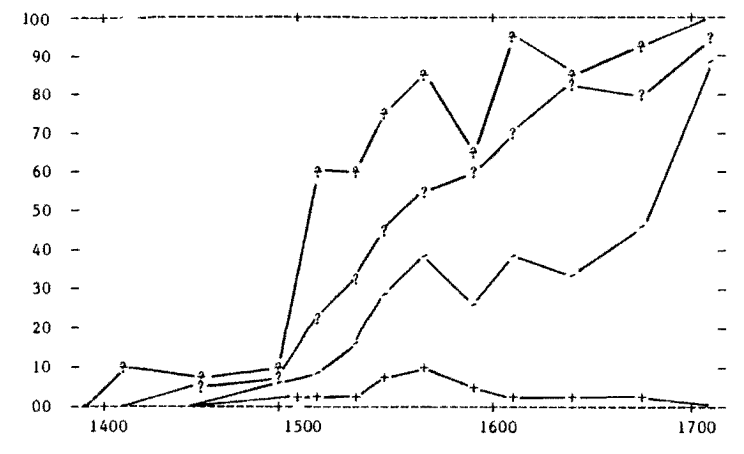
\includegraphics[width=.5\linewidth]{../images/kroch-graph}
		\caption{Frequency of do-support in different environments: affirmative and negative questions (? and \sout{?}) and affirmative and negative declaratives (+ and ') (Fig. 1 from \citealt{Kroch.1989})}
		\label{fig:kroch-graph}
	\end{figure}

	For English `to'-use, there are two changes to be considered (reflecting the rise of the To Grammar and the Allomorphy Grammar). In order to study these changes, I extracted all tokens from the Parsed Corpora of Historical English \citep{Kroch.2000,Taylor.2003,Kroch.2004,Taylor.2006,Kroch.2010} containing the following recipient introducing verbs (verbs that also introduce goals, e.g., SEND, were excluded): ALLOT, APPOINT, ASSIGN, AYEVEN, BEHIEGHT, BEQUEATH, BETAKE, DAELAN, FEED, GIVE, GRANT, LEND, OFFER, OWE, PAY, PROFFER, PROMISE, RESTORE, SELL, SELLAN, SERVE, SHOW, VOUCHSAFE, and YIELD. I also extracted information about whether the arguments were full noun phrases or pronouns, the relative order of the recipient and theme (and their order with respect to the verb to rule out cases of topicalisation), and whether or not the recipient was marked with `to' (passive data was also collected, which is discussed in Section \ref{sec:en-pas}). 
	
	When the theme is a pronoun, the theme--recipient order was essentially categorical (31 examples of recipient--theme order over 1000 years out of 712 examples with theme pronouns). Since there was such poor evidence for the frequency of `to'-use in these environments, their inclusion muddled any attempts at statistical analysis. Therefore, those cases have been excluded for the analyses discussed below.

	In the theme--recipient order, the To Grammar and the Allomorphy Grammar generally produce the same forms. This is because the Allomorphy Grammar only produces a different surface form from the To Grammar when the recipient is adjacent to the verb. In all other cases, the two grammars produce identical surface forms. Since, in theme--recipient orders, the theme intervenes between the recipient and the verb (e.g., ``John gave the book to Mary''), this environment is generally unaffected by the incoming Allomorphy Grammar. The only exception to this is when the theme is a pronoun (as explained in Chapter \ref{ch:active}), since the theme pronoun can cliticise and thus cease to be an intervener.

	\begin{exe}
		\exr{ex:nw-brit-P} Northwestern British English:
		\begin{xlist}
		\ex[ ]{John [gave=it] [P=$\emptyset$ Mary]}
		\ex[*]{John [gave] [the book] [P=$\emptyset$ Mary]}
	\end{xlist}
	\end{exe}

	The aforementioned effects (i.e. the general lack of an effect of the Allomorphy Grammar in the theme--recipient order and the exception when the theme is a pronoun) can be seen in the quantitative data. As can be seen in Figure \ref{fig:brit-tr}, all of the changes show the S-shaped curve that is the predicted outcome of logistic regression (as also seen in Figure \ref{fig:kroch-graph} for the do--support data). However, not all of the curves go to 100\%. When the theme is a pronoun, the curves level out below 100\% (reflecting the effect of theme cliticisation). The rate of `to' use in these contexts (when the theme is a pronoun) reflects the interaction of three properties: (a) the current rate of the To Grammar, (b) the current rate of the Allomorphy Grammar, and (c) the rate of theme cliticisation. Given that there is no independent way of finding the rate of theme cliticisation, cases with a theme pronoun are also excluded from the quantitative analysis below.

	\begin{figure}[ht!]
		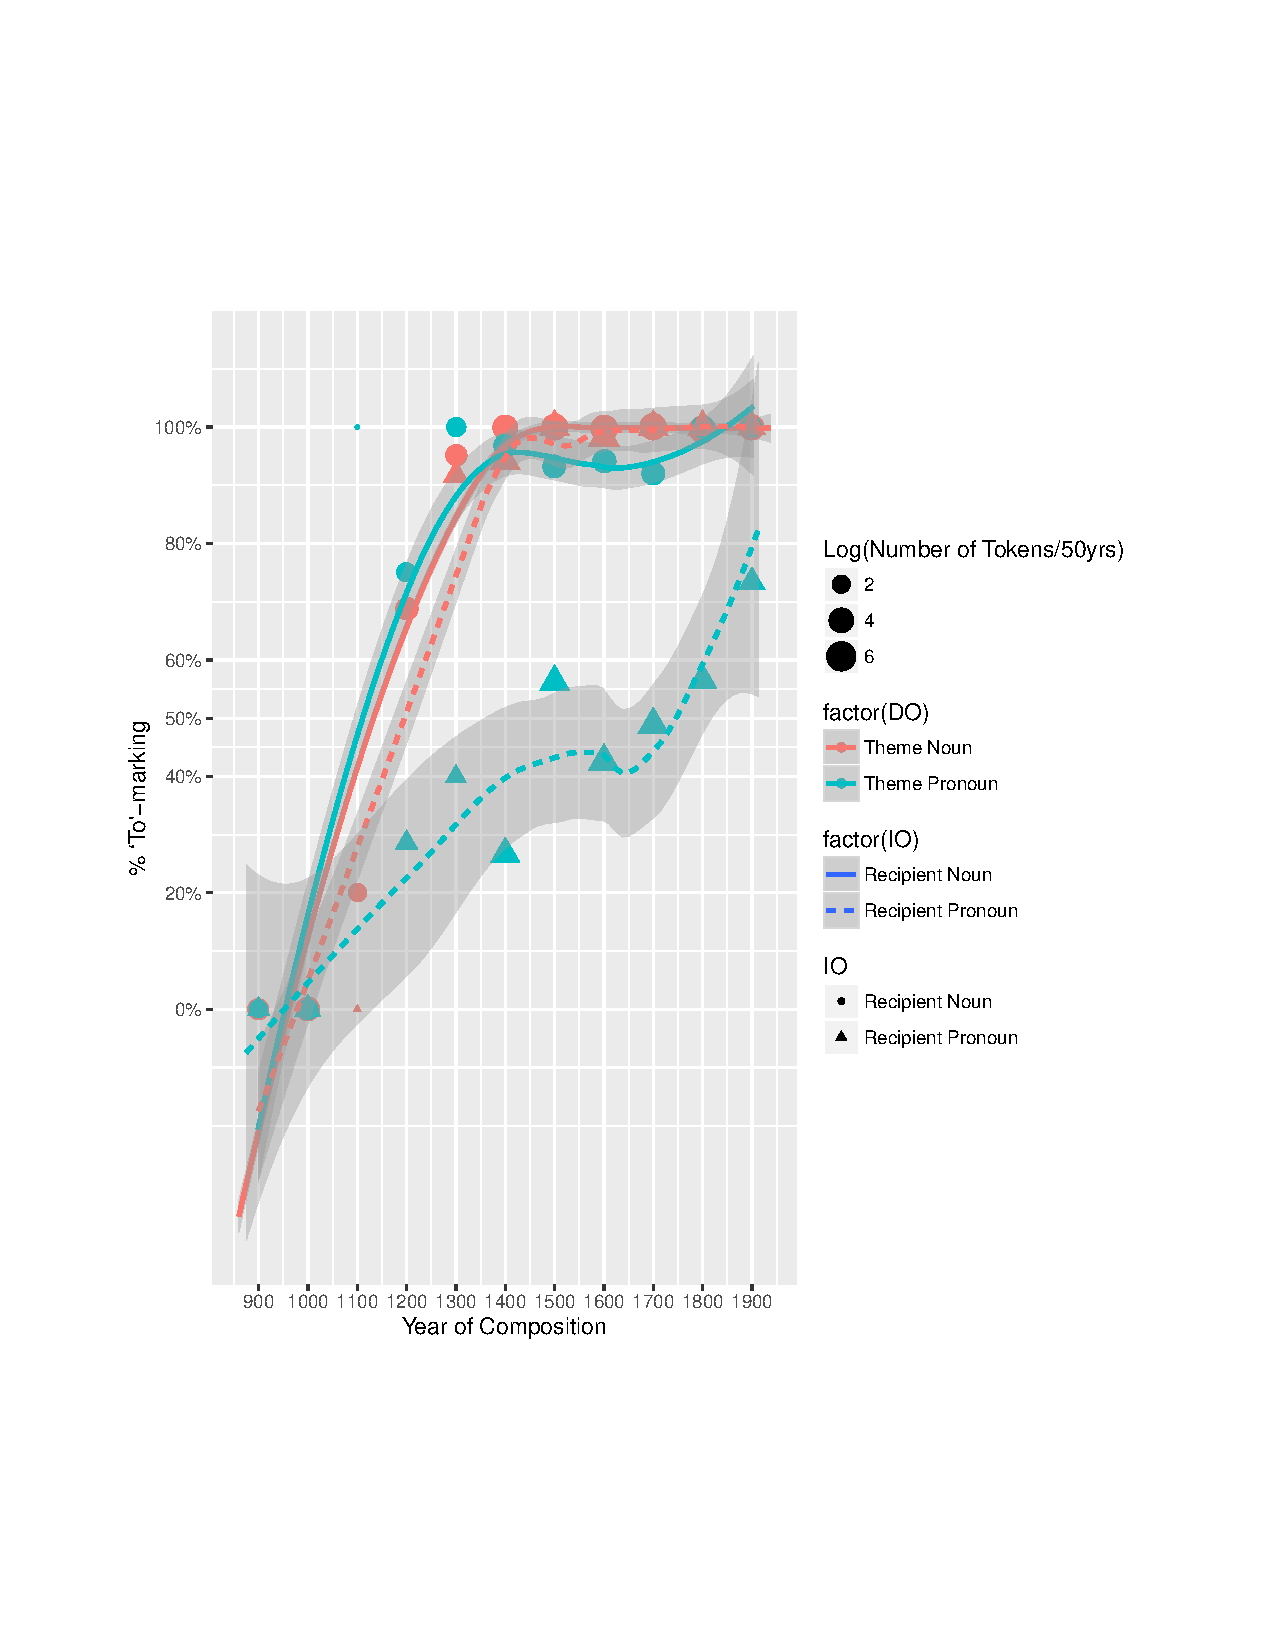
\includegraphics[width=\linewidth]{../images/brit-tr}
		\caption{LOESS fits for theme--recipient data in different combinations of theme and recipient status (points indicate raw frequencies)}
		\label{fig:brit-tr}
	\end{figure}

	Focusing on the data where the theme is a full noun phrase, the effect of the Allomorphy Grammar is clearly seen in the recipient--theme order (without the interfering effect of theme cliticisation). In the recipient--theme order, there is direct competition between the To Grammar and the Allomorphy Grammar as to the realisation of P$_{dative}$ (either as `to' or as $\emptyset$). As can be seen in Figure \ref{fig:brit-tn}, the use of `to' initially rises in the recipient--theme order and then declines. I claim that this rise--fall pattern represents the initial rise from the adoption of the To Grammar, followed by a decline as the Allomorphy Grammar is adopted.

	\begin{figure}
		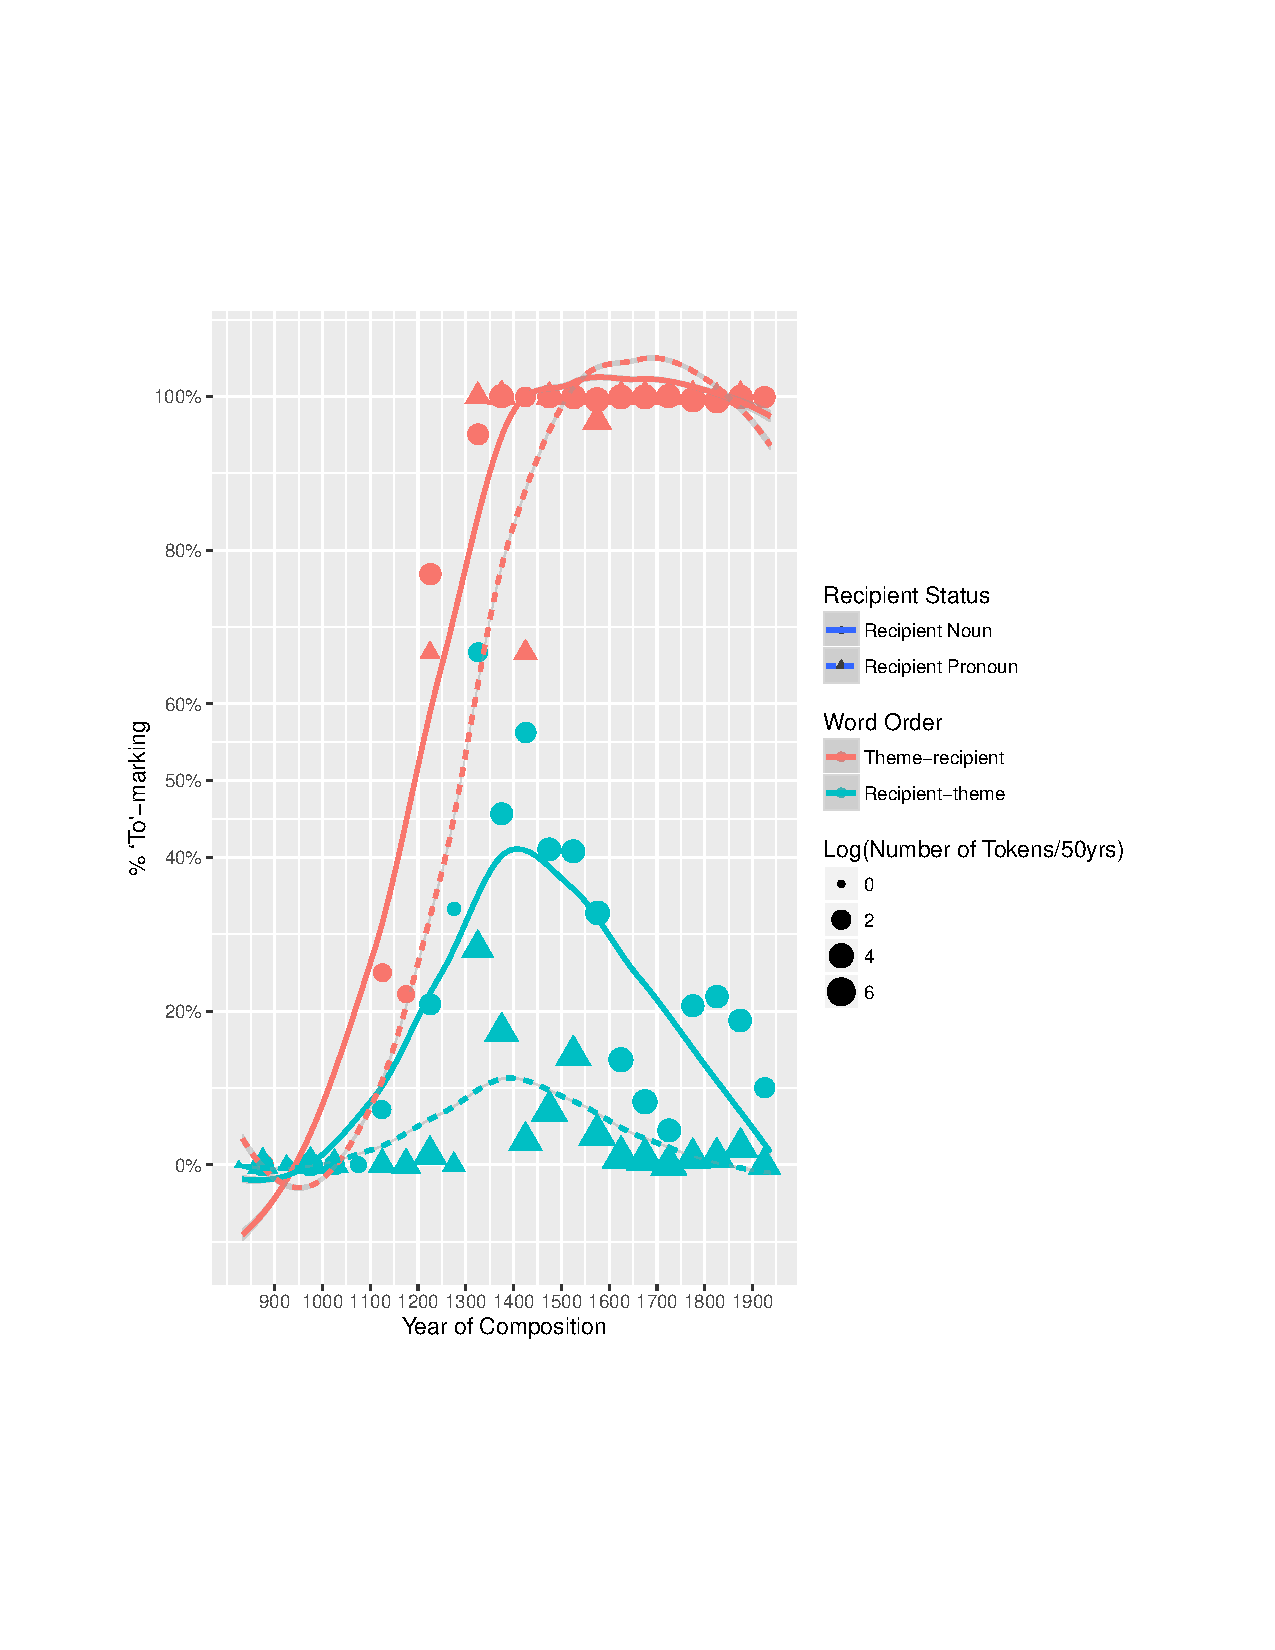
\includegraphics[width=\linewidth]{../images/brit-tn}
		\caption{Model fits for data with full noun phrase theme (points indicate raw frequencies)}
		\label{fig:brit-tn}
	\end{figure}
	
	According to the causal explanation of the Constant Rate Effect (i.e., that the constant rate reflects the rate of adoption of a single underlying grammatical change), a Constant Rate Effect should hold between the rise portion of the recipient--theme data and the rise in the theme--recipient data, since both reflect the underlying adoption of the To Grammar. In order to test the Constant Rate Effect, however, it is necessary to disentangle the role of the To Grammar and the Allomorphy grammar in deriving the rise--fall pattern in the recipient--theme context. 

	The Subset Principle (formally implemented in Distributed Morphology, \citealt{Halle.1993}, but widely accepted in many morphological theories) states: when two forms compete for realisation of the same features, the more specific form is realised. A simple example is the case of irregular verbs, where the irregular rule (e.g., the past tense of `ring' is `rang') beats the more general regular rule (i.e., the past tense of a verb is formed by adding `ed', here leading to `ringed'). In the case of recipient marking, the Subset Principle states that if the Allomorphy Grammar is adopted, then for recipient--theme orders it does not matter whether the Null Grammar or the To Grammar is selected as the general default, the more specific null form will be inserted. However, if the Allomorphy Grammar is \textbf{not} selected, then the choice between the Null Grammar and the To Grammar decides which form gets realised. This can be captured with a 2x2 table reflecting whether the old or innovative form of being used for each change (see Table \ref{tab:2x2int}.


	\begin{table}
		\begin{tabular}{ccc}
					& No Allomorphy Grammar & Allomorphy Grammar\\
			Null Grammar	& John gave him the book & John gave him the book\\
			To Grammar	& John gave \textbf{to} him the book & John gave the book to him\\
		\end{tabular}
		\caption{2x2 table showing the recipient--theme realisation for the interaction between the two changes in dative P realisation in English}
		\label{tab:2x2int}
	\end{table}

	As can be seen in Table \ref{tab:2x2int}, the only way to get `to' in the recipient--theme context is to \textbf{adopt} the To Grammar and \textbf{not} adopt the Allomorphy Grammar. Given that our logistic regression is trying to predict the probability of `to', it is necessary to create a formula that derives the probability of `to' from the interaction of the probability of each change applying. The probability of `to' in the recipient--theme order is equal to the probability of \textbf{both} adopting the To Grammar and not adopting the Allomorphy Grammar. Probability theory states that the probability of two independent events both occurring is equal to the probability of the two events multiplied together. If $p$ represents the probability of adopting the To Grammar and $q$ represents the probability of adopting the Allomorphy Grammar, the probability of not adopting the Allomorphy Grammar is equal to $(1-q)$. Taken together, this means that the probability of `to' in the recipient--theme order is equal to $p * (1-q)$. Both p and q can be modelled with their own logistic function, which means that the Constant Rate Effect can be tested for in each change.\footnote{For details about how the model was fit, see Appendix A for a link to the relevant R files}

	A single model was fit that predicted both the theme--recipient and recipient--theme orders for data with full noun phrase themes using the equation applied above (modified so that q = 0 in the theme--recipient order, so only the p equation would apply). The full model for each change contained effects for year, recipient type, and object order as well as their interactions. The optimal model was selected to have the lowest AIC.\footnote{AIC, Akaike Information Criterion, is a way of selecting models that fit the data well, while taking into account the fact that adding more independent variables always improves fit. Comparing AIC, selects the model that finds an optimal balance between fitting well and having few independent variables.} 
	
	The optimal model had the following properties (model fits shown in Fig. \ref{fig:brit-tn}): (a) the first change was characterised by an intercept, an effect of year, an effect of word order and an effect of recipient status, (b) the second change was characterised by an intercept, an effect of year, and effect of recipient status, and an interaction between year and recipient status. The effects in model (a) indicate a Constant Rate Effect for the introduction of `to'-marking for recipients; there was no significant interaction between conditions. While `to'-marking raises at the same rate across all conditions, recipient--theme orders and recipient pronouns show less `to'-use in any given year. 
	
	As discussed above, failing to find a significant interaction is not enough to automatically claim that the Constant Rate Effect was found, it is possible that there was insufficient data to find a substantial violation of the Constant Rate effect. This explanation for the Constant Rate Effect finding in the first change (adoption of To Grammar) becomes less plausible, given that a significant interaction was identified for the second change (adoption of Allomorphy Grammar) indicating that there was enough data to identify interactions. The identification of a significant interaction for the second change strongly suggests that the Allomorphy Grammar actually reflects two different changes (one for recipient nouns and one for recipient pronouns). The effect of year was found to be higher for recipient pronouns, suggesting that the Allomorphy Grammar affected recipient pronouns faster than full noun phrases (meaning more null forms for pronouns).
	
	Since many languages have a strong differentiation between recipient marking on full noun phrases and pronouns (e.g., Romance language differences between full noun phrases marked with \textit{a} `to' and clitic pronouns marked with synthetic case marking), this differentiation between full noun phrases and pronouns is not unexpected. It appears that there are actually two Allomorphy Grammars: one that applies to nouns, and another that applies to pronouns, which both have the same output, namely $\emptyset$, but which spread through the speech community at different rates. The grammar for pronouns rapidly spread through the speech community (possibly influenced by the fact that pronouns maintained some level of synthetic case marking), while the grammar for full noun phrases spread more slowly. This can be seen in Figure \ref{fig:brit-tn}, where the pronouns show a much less `to' use overall compared to full noun phrases (in recipient--theme word orders).

	By modelling overlapping changes by multiplying their independent probabilities, it was possible to confirm another case of the Constant Rate Effect. In this case, the Constant Rate Effect applied to the rise of the To Grammar. Given that there was independent support that the data was sufficient to detect meaningful interactions, there is solid evidence that the To Grammar was a unified change that applied during the Middle English period. As discussed in Chapter \ref{ch:active}, this supports the dative PP hypothesis by bolstering the notion that the `to' found in the modern theme--recipient orders is actually shared by the recipient--theme order. There was also usage evidence (supporting the judgement data from Northwestern British dialects) that theme cliticisation can license the null allomorph as part of the Allomorphy Grammar.
	
	Looking at the quantitative data also revealed another pronoun related feature of `to' use, namely that there are separate Allomorphy Grammars for full noun phrases and pronouns (i.e., recipient pronouns privilege the null allomorph). Given that Romance clitic pronouns also show different morphological marking from their non-clitic counterparts, this distinction between full noun phrases and pronouns can be viewed as additional evidence for the existence of pronoun specific (i.e., clitic-like) effects in the grammar of Modern British English. Independent evidence about clitic-like effects for both recipients and pronouns increases the likelihood that the theme cliticisation explanation for sentences like (``John gave it him'') are on the right track.

	\section{Passivisation}\label{sec:en-pas}

	This section deals with quantitative data on passivisation with recipient ditransitives, which I argue includes a case of non-grammatical change (i.e., a systematic change in use that does not reflect a change in the underlying grammar). In order to justify this claim, I start by showing that the situation in Old English is ambiguous and thus worth setting aside. I then show two grammatical changes with respect to passivisation of ditransitive recipients: (a) replacement of oblique recipient subjects with nominative recipients and (b) the loss of direct theme passivisation in American English, where direct theme passivisation is reflected in sentences like ``The book was given John''. Finally, I show how the rate of passivisation of ditransitives with recipient--theme word order changes in American English and argue that this change should not be attributed to a change in underlying grammar, but instead to a change in the way speakers choose between multiple possible grammatical utterances. 

\subsection{Old English}
	The situation in Old English is quite complex. \cite{Allen.1999} provides evidence that monotransitive datives are able to become oblique subjects in Old English, but she suggests that in ditransitives, putative oblique subjects are actually topics. To discuss this distinction, she introduces the term ``fronted dative'', which is agnostic as to whether the fronted element is a topic or a subject. The argument about the status of fronted datives in ditransitive passives is made on the basis of Coordinate Subject Deletion facts. In Old English (as in Modern English), arguments are generally obligatory (i.e., neither subject nor object drop is generally licensed). However, when two sentences are coordinated and share the same subject, the subject does not need to be expressed in the second sentence (\ref{ex:OECSD}). In a corpus investigation, none of the fronted datives in ditransitive passives triggered Coordinate Subject Deletion, while a number of fronted nominatives did (see Table \ref{tab:AllenOECSD}). 

	\begin{table}[t]
		\begin{tabular}{cccc}
			Nominative Coreferential & & Deletion & No Deletion \\
			& Order NOM DAT & 11 & 4 \\
			& Order DAT NOM & 4 & 3 \\
			& Total & 15 & 7 \\
			\hline
			Dative Coreferential & & Deletion & No Deletion \\
			& Order NOM DAT & 0 & 27 \\
			& Order DAT NOM & 0 & 11 \\
			& Total & 0 & 38 \\
		\end{tabular}
		\caption{Allen's counts of Coordinate Subject Deletion with ditransitive passive in OE prose (Table 2-6, \citealt{Allen.1999})}
		\label{tab:AllenOECSD}
	\end{table}

	\begin{exe}
		\ex \label{ex:OECSD} Old English:
		\gll and him comon \textbf{englas} to, and him ðenodon\\
		and him.DAT came \textbf{angels.NOM} to, and him.DAT served\\
		\trans ` and to him angels came and him (they) served \citep[ex. 34]{Allen.1999}.''
	\end{exe}

	The main problem with this conclusion is that there were only a small number of Old English coordinated examples, such that the lack of deletion for datives could be accidental. The problem of whether fronted oblique elements are subjects is not unique to Old English. The same uncertainty hold with respect to Old Norse (see for example \citealt{Kristoffersen.1991,Kristoffersen.1994,Bardal.2001b}). Unfortunately, many of the examples that clearly show that oblique elements are subjects rely on negative data, which is unavailable for earlier states of the language. Because of this problem, I focus instead on data starting with Middle English, where I make the assumption that oblique fronted elements are subjects, since Middle English has developed an obligatorily filled subject position.

	\subsection{Changes to Grammar}

	There are two changes going from Early Middle English to Modern American English that affect the grammar of recipient ditransitive passivisation. As discussed in the introduction to this chapter, a grammar distinguishes between strings that are associated with at least one meaning (grammatical strings) and strings that have no association with a meaning (ungrammatical strings). A change to the grammar, thus, means that some strings need to move from one category to another.\footnote{Another type of change in grammar would be a change in the association between meanings among grammatical strings. A grammatical string could be associated with a new meaning, or loose an association with an old meaning, while still being grammatical (i.e., still having some possible interpretations associated with it).} Concerning the passivisation of recipient ditransitives, the two changes are: (a) oblique recipient subjects vs. nominative recipient subjects and (b) availability of direct theme passivisation vs unavailability of direct theme passivisation. 

	As discussed in the previous subsection, I am assuming that Middle English has oblique subjects in cases of fronted recipients. However, since synthetic case marking had been lost (for full noun phrases) by Early Middle English and since the To Grammar (see the previous section) was not yet universal, even with these assumptions, it is difficult to determine whether a fronted recipient was nominative or dative. \cite{Allen.1999}, after carefully examining the extant Middle English corpus, identifies that the first unambiguous case of a nominative recipient subject in the passive of a ditransitive occurs in 1375. This reflects a change in the grammar of English, in so far as previously nominative recipient subjects were ungrammatical and now they are grammatical.

	Under the analysis described in Chapter \ref{ch:passive}, the nature of this grammar change reflects the availability of P-incorporation. Without P-incorporation, the only possible form of recipient passivisation is to have oblique subjects. Given that P-incorporation also generates pseudopassives, the simple prediction would be that pseudopassives would enter the language at the same time as nominative recipient passives. \cite{Sigursson.2014} showed that pseudopassivisation comes into the language in the beginning of the Middle English period. Indeed, as seen in Figure \ref{fig:recpas-pseudo}, pseudopassivisation and nominative recipient passivisation increase in use from about 1200 until 1650, when they both level off.

	\begin{figure}[ht!]
		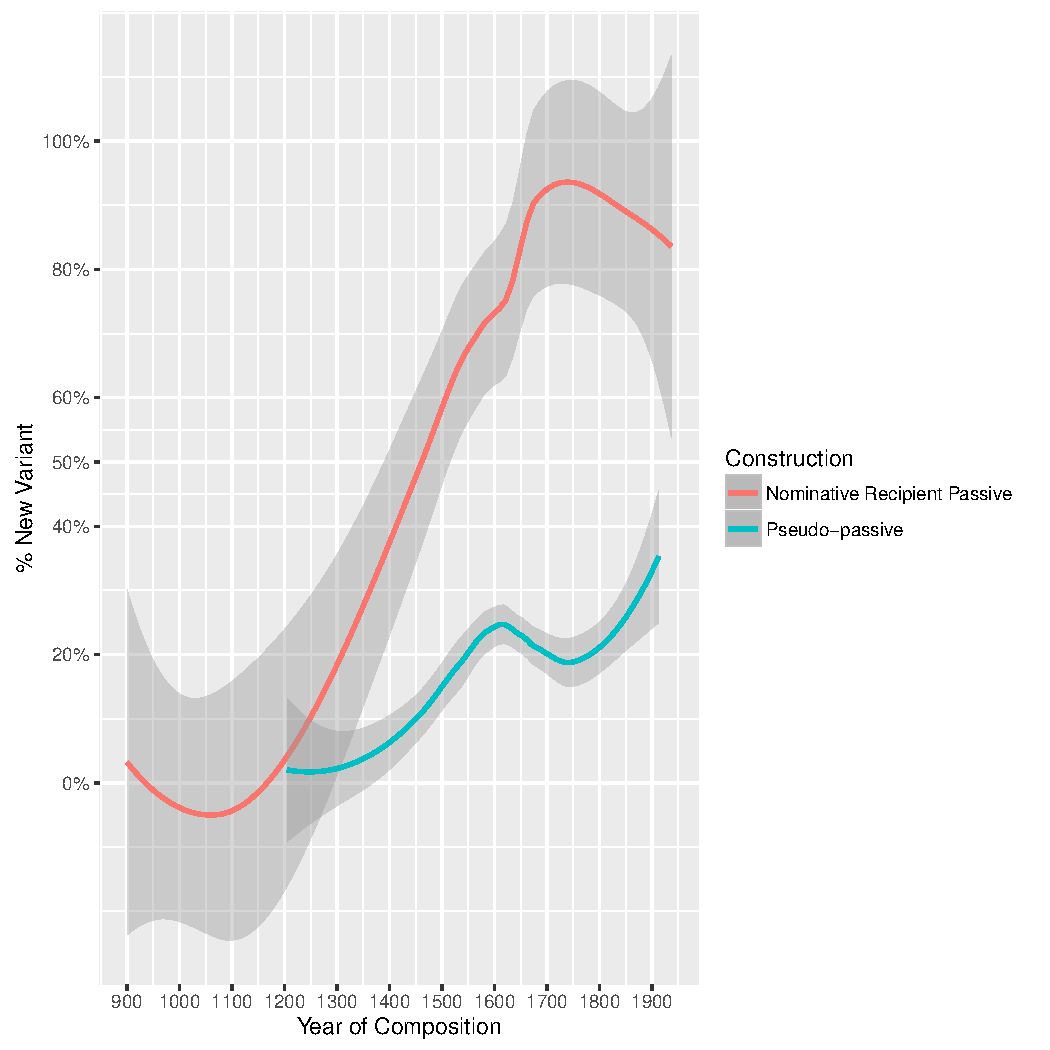
\includegraphics[width=\linewidth]{../images/recpas-pseudo}
		\caption{LOESS curves showing rates of nominative recipient passivisation and pseudopassivisation in English}
		\label{fig:recpas-pseudo}
	\end{figure}

	Neither pseudopassivisation nor nominative recipient passivisation go to 100\%. For pseudopassivisation, this is expected. If the pseudopassivisation rate was 100\% that would mean that there were no active sentences with PP objects, which is highly improbable. For nominative recipient passivisation, it is less clear why the process should not go to completion, since this is the probability of having a nominative subject given that recipient passivisation has occurred, which could reasonably occur 100\% of the time. However, two residual cases prevent this from occurring. Looking at the examples of oblique recipients from the period after 1500, almost all of them are imperatives of the form ``To X, be this given/sent/delivered'', which seem to have been a common formula for deliveries. The other case is locative inversion, for which there is disagreement in the literature about the correct analysis. It seems likely that locative inversion is actually a type of topicalisation and not subject raising \citep{Bresnan.1994}, which means that these cases should actually be excluded (given that they are surface identical to subject raising with oblique dative subjects in these cases, it is impossible to exclude them automatically).

	This would seem to be a good case to look for a Constant Rate Effect (see the previous section). However, there are two problems that prevent looking for a constant rate effect. As can be seen in Figure \ref{fig:recpas-pseudo}, there is a great deal of uncertainty about the rise of nominative recipient passivisation, because there is very little data on recipient passivisation (see the next subsection for a discussion of why there is little data). Thus, even if a Constant Rate Effect was found (i.e., there was no significant interaction between year and pseudopassive vs nominative recipient passive), this could easily be attributed to the lack of data concerning recipient passives. Secondly, the fact that the changes do not go to 100\% means that standard techniques for fitting the logistic regressions cannot be used. Unfortunately, as of this time, I know of no methods for reliably fitting such models. In spite of not being able to quantitatively verify the existence of a Constant Rate Effect, the qualitative similarity in time course between the rise of pseudopassivisation and nominative recipient passivisation supports the notion that they are both derived via the same mechanism (namely P-incorporation).

	The second change in the grammar of ditransitive passivisation occurs within the history of American English. This change is the loss of direct theme passivisation, where the theme raises across the recipient to subject position (for more discussion see Chapter \ref{ch:passive}). In English, direct theme passivisation can be identified by the presence or absence of `to' before the recipient. If the theme scrambles to the left of the recipient before raising to subject position, then its lower copy intervenes between the recipient and the verb, preventing the null allomorph from being used. 

\begin{exe}
	\exr{ex:eng-directtheme} English Dialects:
		\begin{xlist}
			\ex[ ]{The book was given P=$\emptyset$ the man \sout{the book}.}
			\ex[*]{The book was given \sout{the book} P=$\emptyset$ the man \sout{the book}.}
		\end{xlist}
\end{exe}
	
	In Chapter \ref{ch:passive}, direct theme passivisation was argued to result from two possible sources: (a) the locality properties of T in looking for a subject to move (i.e., is a PP in the search domain for subject movement) and (b) recipient pronoun cliticisation. When direct theme passivisation is possible, the recipient is invisible for subject movement either because, as a PP, it is not in the domain of the search (a type of relativised minimality) or because as a clitic it has incorporated into the verbal head. In the new grammar, however, (non-clitic) PPs become defective interveners (i.e., they are not valid targets for the search, but they prevent the search from progressing further down the tree). The loss of direct theme passivisation can be operationalised as both: (a) the replacement of T with the invisible search property with one with defective intervention and (b) the loss of recipient pronoun cliticisation. The trajectory of this change can be seen in Figure \ref{fig:loss-of-dt-in-amen}.

	\begin{figure}[ht!]
		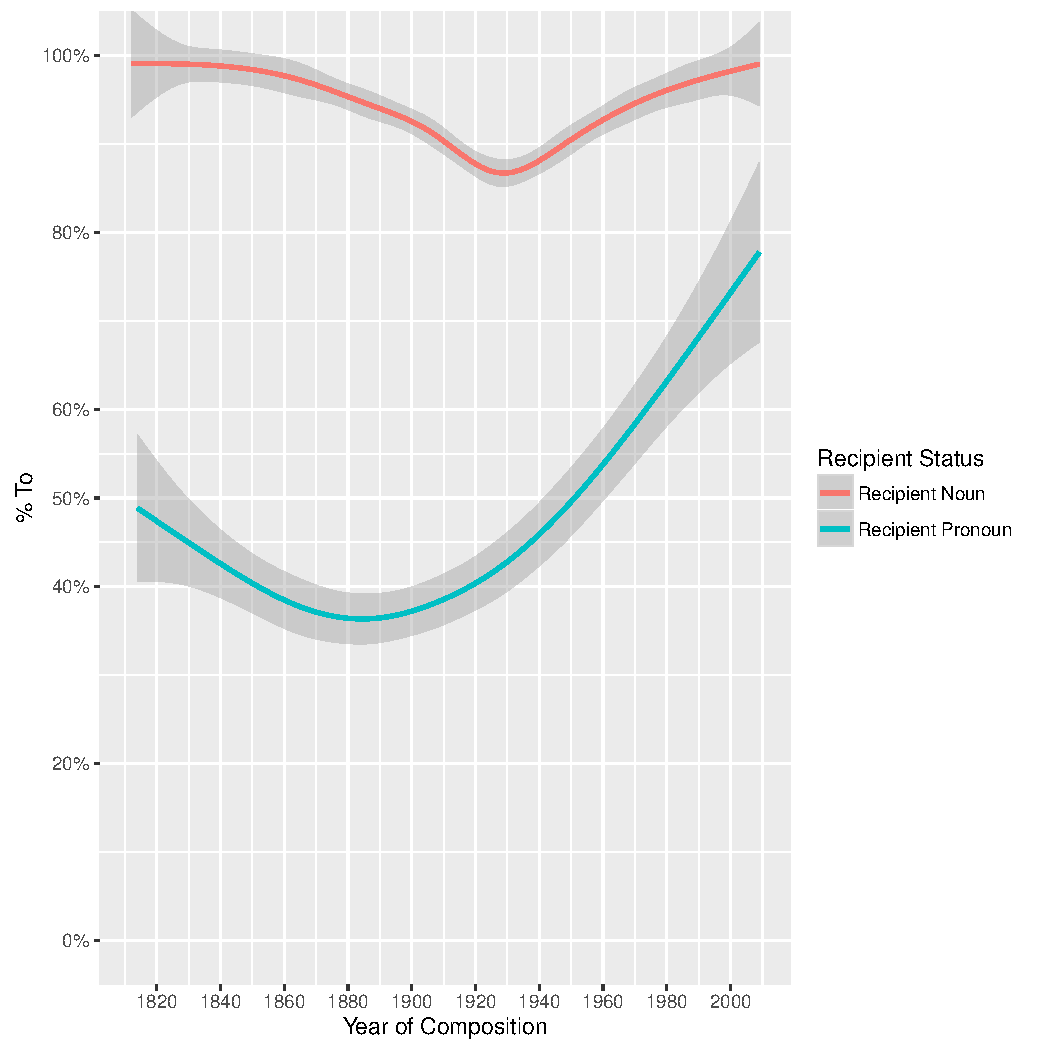
\includegraphics[width=\linewidth]{../images/directtheme-am}
		\caption{LOESS curves showing the loss of direct theme passivisation with GIVE and OFFER in American English}
		\label{fig:loss-of-dt-in-amen}
	\end{figure}

	The change in the locality properties of T and why that might occur is discussed further in the next subsection as part of a discussion of passivisation rates and the interplay between grammar learnability and language production. In particular, I discuss possible non-grammatical reasons for the rise in direct theme passivisation in the late 19th/early 20th century (especially seen with recipient nouns in Figure \ref{fig:loss-of-dt-in-amen}). Before turning to that, it is worthwhile to spend a brief moment on the loss of recipient pronoun cliticisation. As can be seen in Figure \ref{fig:loss-of-dt-in-amen}, direct theme passives are much more common with pronoun recipients than full noun phrase recipients, suggesting that pronoun cliticisation was a common operation that could independently derive direct theme passivisation. The higher rates of direct theme passivisation with recipient pronouns can be directly attributed in this case to the fact that there are two independent mechanisms for generating the same surface phenomenon. In the next subsection, the rate at which these mechanisms are used is discussed.
	
	In Chapter \ref{ch:passive}, I showed that direct theme passivisation survived in American English after the loss of theme cliticisation (i.e., after sentences like ``I gave it him'' became ungrammatical). While the loss of theme cliticisation and the loss of recipient cliticisation were shown to not be identical, there is a plausible connection between the two. It is plausible that language learners generalise evidence about one type of cliticisation, using the evidence of cliticisation with one type of pronoun as supporting evidence for cliticisation with other types of pronouns. Thus, the loss of theme cliticisation removed a potential source of evidence for the existence of cliticisation in the grammar. It is probably not coincidental that direct theme passivisation begins to decline around the same time that theme cliticisation is lost (i.e., 1940s).

	\subsection{Changes in Use of Grammar}

	This subsection discusses a change in American English with respect to the rate of passivisation of ditransitive sentences, especially considering the rates of passivisation of theme--recipient and recipient--theme clauses separately. By passivisation rate for theme--recipient and recipient--theme clauses, I refer to the number of passive sentences with a theme--recipient order (i.e., theme passivisation) out of all theme--recipient sentences (i.e., the number of theme passives divided by the number of theme passives plus the number of theme--recipient actives). For recipient--theme clauses, the same calculation was done, but with recipient passives and recipient--theme actives. In discussing these rates, I start with the end point of the change (i.e., Modern American English), which represents the expected relationship between grammar and use. I then show that this expected relationship is a recent development in the history of English. I then discuss the situation in prior stages of English and argue that is should be accounted for by an non-grammatical mechanism rather than trying to account for the change in patterns with a change in the grammar.

	Assuming that passivisation is pragmatically motivated (probably relating to demotion of agents), it should be expected that passivisation rates should be fairly stable across grammatical contexts. In particular, given that the difference between recipient and theme passivisation does not affect the pragmatic motivation for passivisation (i.e., does not impact the need to demote the subject) and given that both recipient and theme passivisation are grammatical, a naive prediction would be that passivisation rates among recipient--theme and theme--recipient clauses should be roughly equivalent (i.e., the rate of passivisation should be independent of the choice between recipient--theme and theme--recipient word order). Indeed, in late 20th and 21st century American English, this prediction holds; the rate of passivisation in recipient--theme and theme--recipient contexts are roughly equivalent. Collapsing GIVE and OFFER data after 1950, the passivisation rate in recipient--theme contexts is 5.9\%, while the passivisation rate in theme--recipient contest is 5.4\%.\footnote{This result was calculated from the hand-coded data discussed in Chapter \ref{ch:passive} from COHA. The hand coded data included only a sample of active and passive clauses. On the assumption that the sample was representative of the relative portion of recipient--theme and theme--recipient clauses (for both actives and passives), I automatically extracted the number of active and passives sentences with GIVE and OFFER. I then distributed the active and passive sentences into recipient--theme and theme--recipient groups based on the proportions from the hand coded samples. Then passivisation rates for each group was calculated. According to a chi-square test, the two conditions are independent (when looking at the data from 1950 onwards), but there is so much data that essentially any difference would be statistically significant.}
	
	This independence, however, is a new development in the history of English. Early American English and British English (up until the early 20th century) show a lack of independence between passivisation and word order. In particular, passivisation is much rarer in recipient--theme clauses than in theme--recipient clauses with the consequence that recipient passivisation is quite rare. That this property changed in American English can be seen in Figure \ref{fig:am-change-pass}.


	\begin{figure}[ht!]
		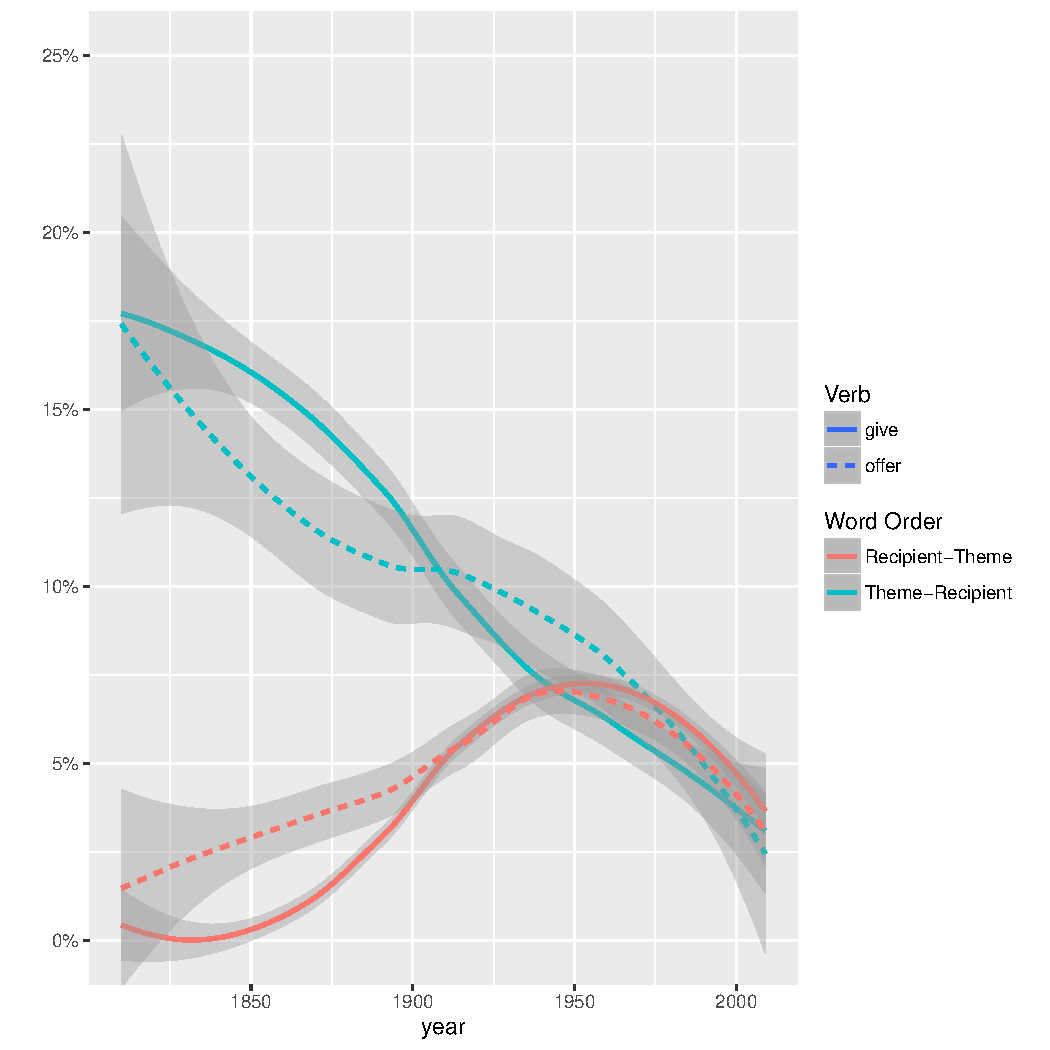
\includegraphics[width=\linewidth]{../images/am-change-pass}
		\caption{Rates of passivisation for GIVE and OFFER from COHA}
		\label{fig:am-change-pass}
	\end{figure}

	This depressed rate of passivisation in recipient--theme clauses has been a long time property of English. Using data from the Parsed Corpora of Historical English discussed in the previous section, the rate of passivisation in recipient--theme clauses was calculated for British English from 1200 (beginning of Middle English) until the 1910s (end of the corpora). The optimal logistic regression model (based on AIC) does not include an effect of year, indicating that the passivisation rate in recipient--theme clauses was stably low ($\sim$1\% of all recipient--theme clauses) for over 700 years. 

	At the same time, passivisation in theme--recipient clauses was consistently (and significantly) higher than in recipient--theme clauses ($\sim$15\% of all theme--recipient clauses). As can be seen in Figure \ref{fig:brit-pas}, the rate in theme--recipient clauses is similar to the general rate of passivisation in the language, which was calculated by dividing the number of passive clauses (excluding pseudopassives) by the number of passive clauses (excluding pseudopassives) plus the number of active clauses with at least one object (i.e., clauses which could have been passivised). Since the passivisation rate in theme--recipient clauses is similar to the general passivisation rate, it is the lower rate in recipient--theme clauses that needs to be explained.

	\begin{figure}[ht!]
		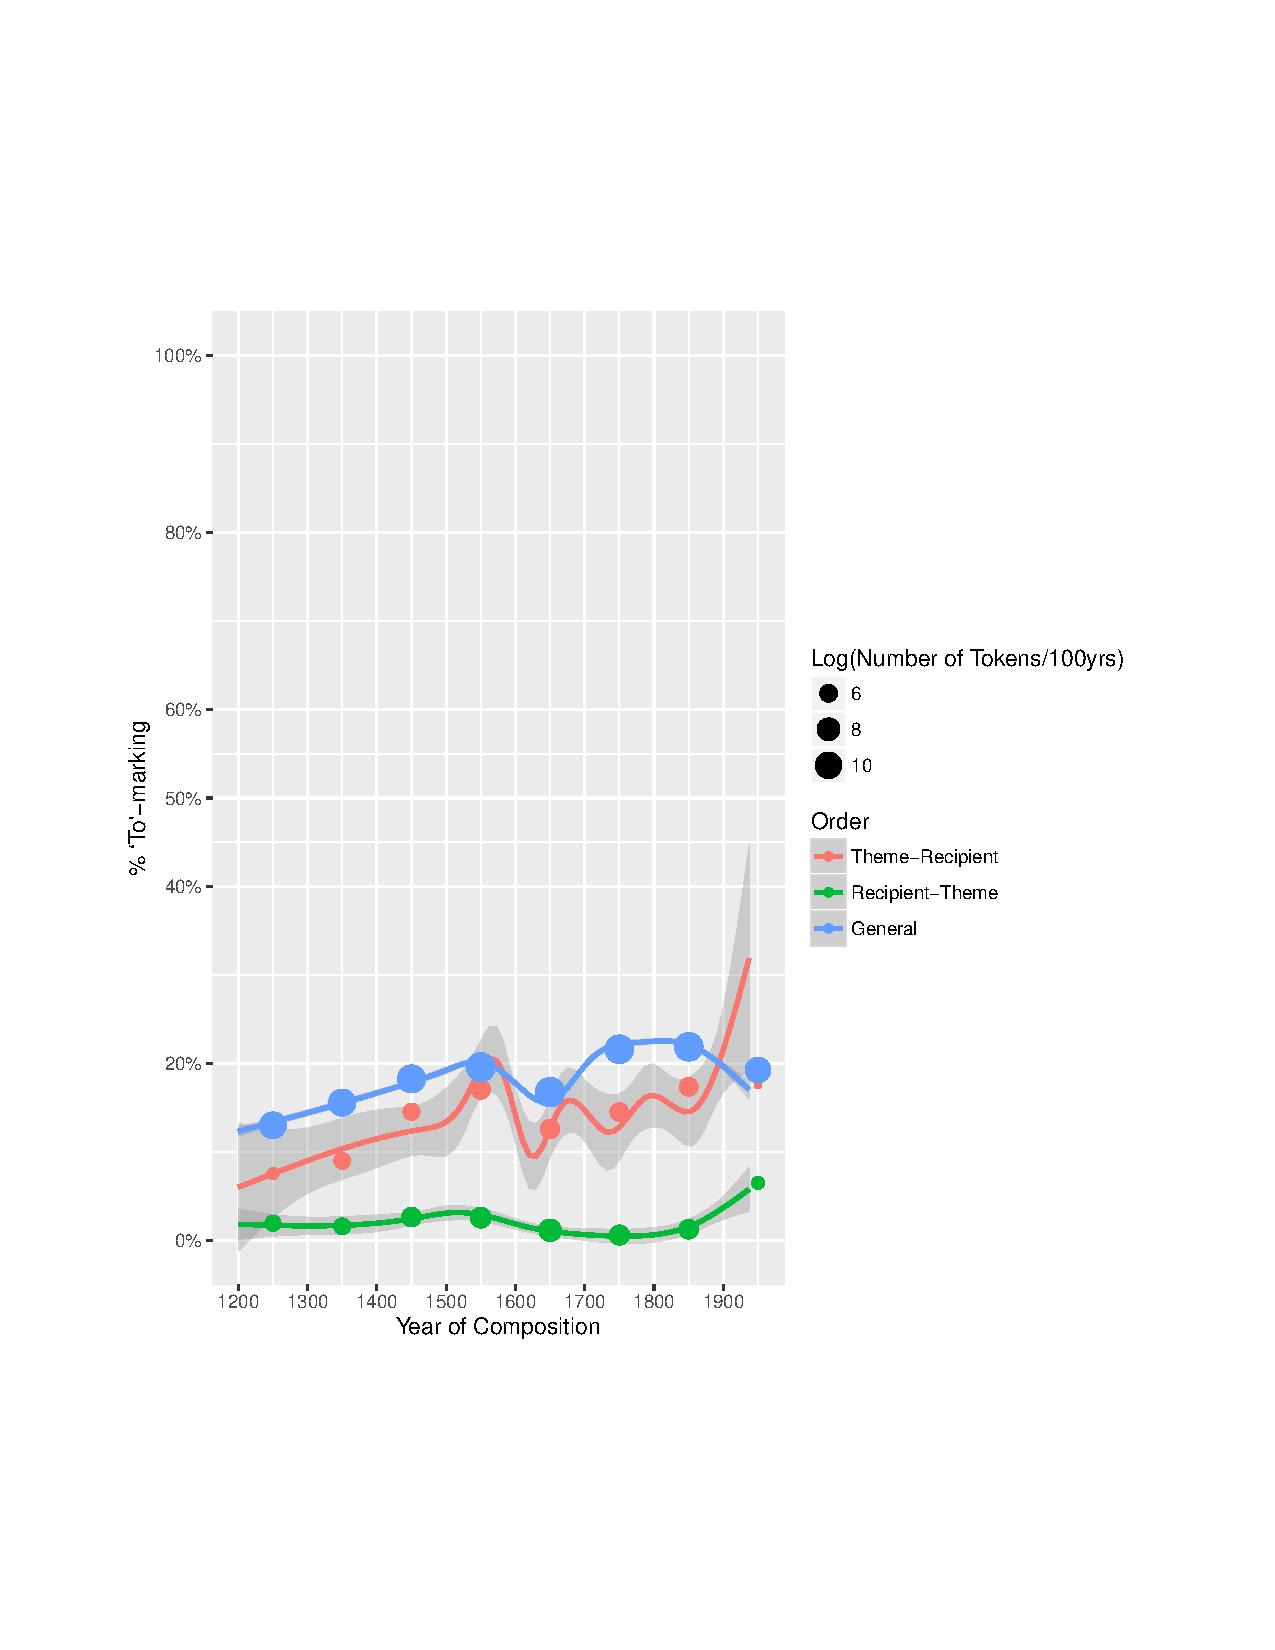
\includegraphics[width=\linewidth]{../images/brit-pas}
		\caption{LOESS fits for rates of passivisation in theme--recipient, recipient theme and general clauses}
		\label{fig:brit-pas}
	\end{figure}

	It would not be simple to provide a grammatical explanation for the phenomenon. In spite of being rarer, recipient passivisation appears to be grammatical (rather than being the artifact of production errors), since an occurrence rate of 1\% seems high for production errors (especially errors involving swapping the position of two arguments). A more complex story would need to claim (as I did in the previous subsection discussing direct theme passivisation) that a difference in rates reflects different derivations for the same string (in the direct passivisation case, the derivations were through relativised minimality and recipient pronoun cliticisation). 
	
	However, passivisation itself is not thought to arise from multiple sources (i.e., it is the effect of a single change in a Voice functional head). In order for different grammatical sources to derive this change, the logic would require that recipient--theme passivisation \textbf{lacks} some passivisation operation that all other clauses share. This is in parallel to the direct theme passive case; direct theme passivisation was higher with recipient pronouns, because there were two different ways of deriving the effect (relativised minimality and recipient pronoun cliticisation). A grammatical explanation of rate differences suggests that higher rates reflects more operations for deriving the relevant construction. Since I already showed that when the rates for recipient--theme passivisation increase in American English, it only increases to become identical to the rates in theme--recipient orders, this would mean that all other passive clauses have some mechanism for passivisation that the recipient--theme order lacks. I am unable to think what such a mechanism would be.

	In addition to not having a viable candidate for a grammatical operation, there is another reason to think that the depressed rate is not grammatical, namely, that the grammar of recipient passivisation changes during the relevant period without affecting the depressed rates. As discussed in the previous subsection, recipient passivisation changed from having oblique recipients to nominative recipients during the period from 1200 to about 1500. At this same time, the rate of recipient passivisation stayed the same. If the rate of recipient passivisation was being driven by grammatical factors, it seems implausible that a change in the relevant grammar would not influence the rate.

	This raises the obvious question: what would a non-grammatical explanation look like? Here is where it is important to separate linguistic competence into grammatical and non-grammatical components. As discussed in the introduction to this chapter, the grammar provides the possibilities to the speaker, but another linguistic component is responsible for determining the probability distribution over those possibilities. Under this conception, the formalisation of the depressed rate is simple: there is an interaction between passivisation and argument order in ditransitives (with passivisation less likely with recipient--theme orders). 

	While this provides a formal mechanism for capturing the phenomenon, it does not constitute an explanation. Why is there such an interaction? What constraints are there on interactions? Are interactions of this type common or rare? While a full discussion of the nature of the probability component would require another dissertation, I include here a brief discussion of possible answers to the first question (the reasons for the interaction). 

	It is worthwhile to note that the marked nature of recipient passives is found across Germanic languages. Icelandic allows theme passivisation even though theme--recipient word orders are ungrammatical in the active. Oblique subjects are extremely rare cross-linguistically, and P-incorporation also appears to be a marked operation (as seen by the rarity of pseudopassivisation). Language users seem to prefer to not manipulate PPs in order to have them become subjects. In cases where there is no other alternative (e.g., pseudopassives), speakers use P-incorporation to accomplish their goals. However, when there are other options available (e.g., theme passivisation for ditransitives), speakers avoid using a grammatical alternative involving manipulating a PP unless other factors (e.g., information structure) force them to use P-incorporation (or allow oblique subjects). 

	Returning to direct theme passivisation can give some further insight into the nature of the formal interaction. Since direct theme passivisation is (by definition) theme passivisation from the recipient--theme order, it should fall under the scope of the interaction (i.e., it should also show a decreased rate). Indeed, direct theme passivisation with full noun phrase recipients is quite rare (~2\% of all theme passives with full noun phrase recipients). However, direct theme passivisation is quite common with pronominal recipients (~50\% of all theme passives with pronominal recipients). This discrepancy in rates between full noun phrases and pronouns is informative about what triggers the interaction (i.e., non-cliticised recipients adjacent to the voice morpheme).

	In addition, the change in the non-grammatical system for determining passivisation rates for recipient--theme clauses explains the initial rise in direct theme passivisation in late 19th and early 20th century American English (shown in the previous subsection). Since direct theme passivisation (especially with full noun phrase recipients) derives from passivisation of recipient--theme clauses, increase in the rates of recipient--theme clause passivisation also increases the rate of direct theme passivisation. Possibly, the subsequent decline of direct theme passivisation with full noun phrase recipients is driven by the grammatically unrelated decline in direct theme passivisation with recipient pronouns. That decline was attributed to a loss of recipient cliticisation, but language learners may have overgeneralised the loss to apply to all sources of direct theme passivisation.

\section{Conclusions}
	In this chapter, I showed examples of using quantitative studies in syntactic change to inform linguistic research. This was embedded in a discussion of the nature of linguistic architecture and the relevance of different types of linguistic evidence. Examples were brought to show that quantitative use data can be informative about grammar, but is essential in studying systematic non-grammatical aspects of language.
	
	Looking at the development of recipient marking in English (i.e., the innovation of `to' as the marker of recipients) provided an example of how even complex changes involving the interaction of two distinct changes can be broken apart using relatively simple statistical processes. By breaking apart interacting changes, it is possible to use quantitative measures (such as the Constant Rate Effect) to study the grammatical architecture underlying each change. In this case, the initial rise of `to' as a marker of recipients showed a Constant Rate Effect implying that there was one underlying `to' grammar. On the other hand, the development of a null allomorph (used when the recipient is adjacent to the verb) showed a significant interaction between year and recipient status (pronoun vs. noun), indicating that the null allomorphy reflects different underlying grammars for nouns and pronouns. While this finding is not surprising, given the already known differences between nouns and pronouns in English morphology, it could not have been discovered without looking at quantitative data.
	
	Looking at passivisation, another case of a clear grammatical change was identified. In particular, both nominative recipient passivisation and pseudopassivasition increase in use during the same time period (Middle and Early Modern English). In this case, there was insufficient data to get quantitative results, but the qualitative overlap gives tentative support to the notion that both nominative recipient passivisation and pseudopassivisation are driven by the same mechanism (namely P-incorporation).

	Finally, the second case study also provided some insight into the underlying mechanism driving changes in use frequency of syntactic mechanisms. In at least some cases, it is the mechanism for determining probability distributions for production that is subject to change. In this case, passivisation was less likely in recipient--theme clauses (independently of whether the passivisation would produce an oblique recipient subject, a nominative recipient subject or direct theme passivisation). This restriction was stable for almost 700 years, but in American English was lost in favour of the simpler system with a uniform passivisation rate across environments. This provided evidence for a non-grammatical component to language competence (a system for determining probabilities for production), which can most profitably be studied using corpora of production.

%\bibliography{diss}
